
%% bare_adv.tex
\documentclass[10pt,journal,twoside]{IEEEtran}

% Some very useful LaTeX packages include:

% *** CITATION PACKAGES ***
%
\ifCLASSOPTIONcompsoc
  \usepackage[nocompress]{cite}
\else
  \usepackage{cite}
\fi
% *** GRAPHICS RELATED PACKAGES ***
%
\ifCLASSINFOpdf
   \usepackage[pdftex]{graphicx}
\else
   \usepackage[dvips]{graphicx}
\fi
% *** MATH PACKAGES ***
%
\usepackage{amsmath}
% *** SPECIALIZED LIST PACKAGES ***
\usepackage{acronym}
\usepackage{algorithmic}
% *** ALIGNMENT PACKAGES ***
%
\usepackage{array}
% *** SUBFIGURE PACKAGES ***
\ifCLASSOPTIONcompsoc
 \usepackage[caption=false,font=footnotesize,labelfont=sf,textfont=sf]{subfig}
\else
 \usepackage[caption=false,font=footnotesize]{subfig}
\fi
% *** FLOAT PACKAGES ***
%
\usepackage{fixltx2e}
% *** PDF, URL AND HYPERLINK PACKAGES ***
%
\usepackage{url}

% NOTE: PDF hyperlink and bookmark features are not required in IEEE
%       papers and their use requires extra complexity and work.
% *** IF USING HYPERREF BE SURE AND CHANGE THE EXAMPLE PDF ***
% *** TITLE/SUBJECT/AUTHOR/KEYWORDS INFO BELOW!!           ***
\newcommand\MYhyperrefoptions{bookmarks=true,bookmarksnumbered=true,
pdfpagemode={UseOutlines},plainpages=false,pdfpagelabels=true,
colorlinks=true,linkcolor={black},citecolor={black},urlcolor={black},
pdftitle={Nayem_DraftTASLP},%<!CHANGE!
pdfsubject={Typesetting},%<!CHANGE!
pdfauthor={Khandokar Md. Nayem},%<!CHANGE!
pdfkeywords={TASLP, journal, LaTeX, paper,
             template}}%<^!CHANGE!
\ifCLASSINFOpdf
\usepackage[\MYhyperrefoptions,pdftex]{hyperref}
\else
\usepackage[\MYhyperrefoptions,breaklinks=true,dvips]{hyperref}
\usepackage{breakurl}
\fi

\usepackage{booktabs}
\usepackage{multirow}
\usepackage{adjustbox, bm}
\usepackage{xcolor}
\usepackage{pgfplots}
% \pgfplotsset{compat=1.15}
\pgfplotsset{compat = 1.9}
\usepgfplotslibrary{colorbrewer}
\usetikzlibrary{pgfplots.statistics, pgfplots.colorbrewer} 
\usepackage{tikz}
\usepackage{amsfonts}
\usepackage{pgfplotstable}
\usepackage{filecontents}

% limits underneath
\DeclareMathOperator*{\argmax}{arg\,max\,}
\DeclareMathOperator*{\argmin}{arg\,min\,}

\newcommand\mytodo[1]{\textcolor{red}{#1}}
\newcommand\nayem[1]{\textcolor{blue}{#1}}

% correct bad hyphenation here
\hyphenation{op-tical net-works semi-conduc-tor}


\begin{document}
%
% paper title
\title{Attention-based Speech Enhancement Using Human Quality Perception Modelling}
%
%
% author names and IEEE memberships
\author{Khandokar~Md.~Nayem,~\IEEEmembership{Student Member,~IEEE,}
        and~Donald~S.~Williamson,~\IEEEmembership{Senior Member,~IEEE}% <-this % stops a space

\thanks{This work was supported in part by NSF under Grant IIS-1942718 and in part by Lilly Endowment, Inc., through its support for the Indiana University Pervasive Technology Institute}%     
\thanks{Khandokar Md. Nayem is with the Department of Computer Science, Indiana University, Bloomington, IN 47408 USA (e-mail: knayem@iu.edu).}%

\thanks{Donald S. Williamson was with the Department of Computer Science at Indiana University, but he is now with the Department of Computer Science and Engineering, Ohio State University, Columbus, OH, USA 43210 USA (e-mail: 
williamson.413@osu.edu).}%

% \thanks{Digital Object Identifier ***}
}



% The paper headers
% \markboth{IEEE/ACM~TRANSACTIONS~ON~AUDIO,~SPEECH,~AND~LANGUAGE~PROCESSING,~Vol.~0, No.~0, Mar~2023}%
% {NAYEM~AND~WILLIAMSON:~Attention-based~Speech~Enhancement~Using~Human~Quality~Perception~Modelling}
% The only time the second header will appear is for the odd numbered pages
% after the title page when using the twoside option.



\IEEEtitleabstractindextext{%
\begin{abstract}
Perceptually-inspired objective functions such as the perceptual evaluation of speech quality (PESQ), signal-to-distortion ratio (SDR), and short-time objective intelligibility (STOI), have recently been used to optimize performance of deep-learning-based speech enhancement algorithms. These objective functions, however, do not always strongly correlate with a listener's assessment of perceptual quality, so optimizing with these measures often results in poorer performance in real-world scenarios. In this work, we propose an attention-based enhancement approach that uses learned speech embedding vectors from a mean-opinion score (MOS) prediction model and a speech enhancement module to jointly enhance noisy speech. The MOS prediction model estimates the perceptual MOS of speech quality, as assessed by human listeners, directly from the audio signal. The enhancement module also employs a quantized language model that enforces spectral constraints for better speech realism and performance. We train the model using real-world noisy speech data that has been captured in everyday environments and test it using unseen corpora. The results show that our proposed approach significantly outperforms other approaches that are optimized with objective measures, where the predicted quality scores strongly correlate with human judgments. 
\end{abstract}

% Note that keywords are not normally used for peerreview papers.
\begin{IEEEkeywords}
speech enhancement, speech quantization, speech assessment, attention model, deep learning, speech quality.
\end{IEEEkeywords}}

% make the title area
\maketitle



\IEEEdisplaynontitleabstractindextext
\IEEEpeerreviewmaketitle

%%%%%%%%%%%%%%%%%%%%%%%%%%%%%%%%%%%%%%%%%%%%%%%
%%%%%%%            SECTIONS             %%%%%%%
%%%%%%%%%%%%%%%%%%%%%%%%%%%%%%%%%%%%%%%%%%%%%%%
\section{Introduction}
\label{sec:intro}
\begin{figure}[t]
\begin{center}
    \includegraphics[width=1\linewidth]{figures/teaser.pdf}
\end{center}
\vspace{-0.1in}
\caption{\textbf{{\em Foggy} vs {\em Clear} NeRF.} Our \ournerf gets rid of reconstruction errors manifested as foggy ``floaters" in the density volume without additional input or significant computational overhead. 
%
Below are density profiles along a given ray before and after our geometry correction procedure, where we discard density peaks corresponding to floaters.
}
\label{fig:teaser}
\vspace{-0.2in}
\end{figure}



%The emergence of 
Neural Radiance Fields (NeRFs)~\cite{mildenhall2020nerf}  %and its variants 
have made revolutionary contributions in %photo-realistic 
novel view synthesis~\cite{barron2021mip,barron2022mip}, 
autonomous driving~\cite{rematas2022urban,tancik2022block}, digital human~\cite{hong2022headnerf,zhao2022humannerf}, and 3D content generation~\cite{eg3d,poole2022dreamfusion,lin2022magic3d}.
%by leveraging a multi-layer perceptron (MLP) to implicitly model the mapping from input 5D coordinates (i.e., 3D coordinates $\mathbf{x} = (x,y,z)$ and 2D viewing directions $\mathbf{d}=(\theta,\phi)$) to volume density $\sigma$ and view-dependent emitted radiance color $\mathbf{c} = (r,g,b)$. 
%
%They then use traditional volume rendering mechanisms on the obtained continuous 5D function (i.e., MLP) to generate novel views. 
To date, unfortunately, most NeRF-based methods encounter challenges when tackling large-scale cluttered scenes (e.g., Fig.~\ref{fig:teaser}):
\begin{enumerate}[leftmargin=0.16in, topsep=2pt,itemsep=-1ex,partopsep=1ex,parsep=1ex]
\item Input observations used for NeRF are often too sparse  compared to forward-facing or synthetic looking-inward scenes;
%\item Recovering fine-grained objects within a large volume is challenging for NeRF; %in capturing details accurately.
\item View-dependent visual effects give rise to ambiguity, resulting in a ``foggy" density field as shown in Fig.~\ref{fig:teaser}. 
%
Such artifacts are particularly pronounced in indoor scenes strewn with view-dependent appearances, such as specular highlights, glossy surface reflections from man-made objects. 
\end{enumerate}

Despite attempts to enhance NeRF's rendering quality given suboptimal input, such as using 3D conical frustums~\cite{barron2021mip,barron2022mip}, physically-grounded augmentations~\cite{chen2022aug}, and misalignment correction~\cite{jiang2022alignerf},  these challenges have yet to be fully resolved.
%
Depth supervision~\cite{deng2022depth, wei2021nerfingmvs} or proxy geometry~\cite{xu2021scalable,wu2022scalable} images can help alleviate the challenges in handling large-scale with sparse input, at the expense of %but they come at the cost of requiring 
expensive pre-processing or additional input.
%
Another line of work~\cite{wang2021neus, oechsle2021unisurf, wang2022neuris} achieves better reconstruction of surface geometry by using signed distances instead of volume density as scene representation. However, they sacrifice the ability to synthesize photo-realistic novel views.

%We observe that NeRF has been suffering from foggy ``floater" artifacts in large-scale cluttered scenes.
%
%Such artifacts are particularly pronounced in indoor scenes strewn with view-dependent appearances from man-made objects. 
%
To address the above issues, we propose an extension to NeRF, dubbed as {\bf \ournerf}, which enforces effective {\em appearance} and {\em geometry} constraints conducive to accurate colors and 3D densities estimation. We believe \ournerf can contribute beyond novel view synthesis, such as NeRF object detection~\cite{hu2022nerf}, NeRF object segmentation~\cite{zhi2021place, liu2022unsupervised, fan2022nerf,ren2022neural}, and NeRF registration~\cite{goli2022nerf2nerf}, where the rooms for improvement are substantial if more accurate color and density estimation are available.

Correspondingly, there are two steps in \ournerf. First, for appearance correction, the view-independent and view-dependent color components are predicted from the underlying 3D scene, which is combined to produce the final color estimation (Fig.~\ref{fig:toaster}).
%
The view-independent component (diffuse color and shading) captures the overall scene color, while the view-dependent component (highlights or reflections) captures color variations due to changes in viewing angle.
%
\ournerf then discards these view-dependent appearances in the training views to prevent them from interfering with the density estimation.
%
Second, a simple and effective geometry correction procedure will be performed to further eliminate the foggy ``floaters" or density errors. This geometry correction procedure is based on an assumption in line with traditional ray tracing in computer graphics.
\begin{comment}
% xh: basically copying method
On the other hand, ClearNeRF performs a geometric correction procedure performed on each traced ray during inference to refine the density estimation and better tackle the floater artifacts. 
%
The geometry correction procedure assumes that there should only be one salient peak along each traced ray during NeRF inference. 
Only the salient peak closest to the ray origin (the camera center) corresponds to  true geometry while the others will be manifested as foggy floaters hovering in the density volume. 
%
This assumption is in line with traditional ray tracing in computer graphics where in the absence of noise, only one intersection per ray should be returned to indicate the closest ray-object intersection.
%
\end{comment}
%%%%%%%%%%%
%As shown in Fig.~\ref{fig:teaser}, when reconstructing an indoor scene with sparse input and highly view-dependent objects, NeRF produces severe floating artifacts due to its attempt to explain view-dependent appearances.
%
Experiments verify that our proposed \ournerf can effectively get rid of floater artifacts without additional input.% or significant computational overhead. 


In summary, our contributions include the following:
\begin{itemize}[leftmargin=0.16in, topsep=2pt,itemsep=-1ex,partopsep=1ex,parsep=1ex]
    \item We propose a concise method for decomposing view-independent and view-dependent appearance during NeRF training and eliminate the interference of view-dependent appearance.
    \item We propose a geometric correction procedure performed on each traced ray during inference to refine the density estimation and better tackle the floater artifacts.
    \item Extensive experiments and ablations verify the effectiveness of our core designs and results in improvements over the vanilla NeRF and other state-of-the-art alternatives.
    %without additional computational resources or other inputs.
\end{itemize}




%%%%%%%%%%%%%%%%%%%%%%%%%%%%%%%%%%%%%%%%%%%%%%%
%%%%%%%        2. Proposed Approach         %%%%%%%
%%%%%%%%%%%%%%%%%%%%%%%%%%%%%%%%%%%%%%%%%%%%%%%

\section{Proposed Approach}
\label{sec:methods}

A depiction of our approach is shown in Figure \ref{fig:model}. The model consists of a MOS prediction model (shown left) and a speech enhancement model (shown right). Our MOS prediction model is tailored to provide estimates for subjective-MOS (as rated by humans), and going forward, we will use MOS to refer to subjective-MOS unless explicitly stated otherwise, for ease of understanding. We next will provide notation and then describe each of these sub-modules.

\subsection{Notation}

We define a clean speech signal as $s_t$ and background noise as $n_t$ at time $t$. The mixture of clean speech and noise is denoted as $m_t=s_t+n_t$. We aim to extract the speech from the mixture by removing the unwanted noise. The short-time Fourier transform (STFT) converts the time-domain mixture into a T-F representation, $M_{t,f}$, that is defined at time $t$ and frequency $f$. The complex-valued STFT matrix, $\bm{M}$, can be written as $\bm{M}=|\bm{M}|e^{i\bm{\theta}^M}$ with magnitude $|\bm{M}|\in \bm{\Re}^{T\times F}_+$ and phase $\bm{\theta}^M \in \bm{\Re}^{T\times F}$, where $T$ is the length of speech in time and $F$ is the total number of frequency channels.

Enhancing the magnitude response of noisy speech results in an estimate of the clean speech magnitude response, $|\hat{\bm{S}}|$, using an enhancement function $\mathcal{F}_\delta$ such that $|\hat{\bm{S}}| =\mathcal{F}_\delta(|\bm{M}|)$. The enhancement function is modeled with a deep neural network which is trained to maximize the conditional log-likelihood of the training dataset, 
\begin{align*}
    &\max \frac{1}{N} \sum^N \log P\Big( |{\bm{S}}| \, \Big| \, |\bm{M}|\Big) \\
    \Rightarrow &\max_\delta \frac{1}{N} \sum^N \log P\Big( \mathcal{F}_\delta(|\bm{M}|) \, \Big| \, |\bm{M}|\Big)
\end{align*}
% $$\max \frac{1}{N} \sum^N \log P\Big( |{\bm{S}}| \, \Big| \, |\bm{M}|\Big) \Rightarrow \max_\delta \frac{1}{N} \sum^N \log P\Big( |\hat{\bm{S}}| \, \Big| \, |\bm{M}|\Big) $$
where $\delta$ denotes the set of tunable parameters and $N$ is the number of training examples. The estimated magnitude response $|\hat{\bm{S}}|$ is then combined with the noisy phase, $\bm{\theta}^M$, where the inverse STFT produces an enhanced speech signal in the time domain, $\hat{s}_t$. 

\subsection{Speech quality assessment model}
\label{subsec:mos_model}

A MOS prediction model proposed by \cite{dong2020pyramid} is adapted to estimate the MOS from noisy speech. This model has been developed with real-world captured data and it has been shown to outperform comparison approaches~\cite{fu2018quality, avila2019non, mittag2019non}, according to multiple metrics. The MOS prediction model consists of an attention-based encoder-decoder structure that uses stacked pyramid bi-directional long-short term memory (pBLSTM)~\cite{chan2016listen} networks in the encoder. We denote this model as Pyramid-MOS (PMOS). A pBLSTM architecture gives the advantages of processing sequences at multiple time resolutions, which effectively captures short- and long-term dependencies. Speech has spectral and temporal dependencies over short and long durations, and a multi-resolution framework is effective in learning these complex relations. 


A single T-F frame of the noisy-speech mixture, $|\bm{M}_t|$, is the input to the PMOS encoder. In a pyramid structure, the lower layer outputs from $\Upsilon$ consecutive time frames are concatenated and used as inputs to the next pBLSTM layer, along with the recurrent hidden states from the previous time step. The output of a pBLSTM node is an embedding vector, $h^l_t$, that is as defined below:
\begin{align}
    h^l_t &= pBLSTM\Big( h^l_{t-1}, \big[ h^{l-1}_{\Upsilon\times t -\Upsilon+1}, h^{l-1}_{\Upsilon\times t}\big] \Big)
\end{align}
where $\Upsilon$ is the reduction factor (e.g., number of concatenated frames) between successive pBLSTM layers and $l$ is the layer number. A pBLSTM reduces the time resolution from the input speech to the final latent representation $\bm{H}$. Figure~\ref{fig:pBLSTM} shows the internal structure of pBLSTM module.
This compressed vector accumulates the useful features for measuring speech perceptual quality that resides in a range of time-frames and ignores the least important features.
The encoder outputs a concatenated version of the hidden states of the last pBLSTM layer as vector $\bm{H}=\{\bm{h}_1, \dotsb, \bm{h}_\tau, \dotsb, \bm{h}_\wp\}$, where $\wp$ is the total number of final embedding vectors with time index $\tau$.

The output of the PMOS encoder becomes the input to the PMOS decoder unit. This decoder is implemented as an attention layer followed by a fully-connected (FC) layer and it outputs an estimated MOS of the input speech utterance. Attention models learn key attributes of a latent sequence, since adjacent time frames can provide important information, which is particularly crucial for our task.  
The attention mechanism~\cite{luong2015effective} uses the pyramid encoder output at the $i$-th and $k$-th time steps to compute the attention weights, $\alpha^{PMOS}_{i,k}$. Attention weights are used to compute a context vector, $c^{PMOS}_i$, using the following equations:
\begin{align}
    \alpha^{PMOS}_{i,k} &= \frac{\exp{(\bm{h}_i^\top \bm{Q} \bm{h}_k)}}{\sum^{\wp}_{\phi=1} \exp{(\bm{h}_i^\top \bm{Q} \bm{h}_\phi)}}\\
    % \alpha^{PMOS}_{i,k} &= Attention(\bm{h}_i, \bm{h}_k)\\
    c^{PMOS}_i &= \sum^\wp_{k=1} \alpha^{PMOS}_{i,k} \cdot \bm{h}_k
\end{align}
$\bm{Q}^{\wp\times\wp}$ is the trainable PMOS attention weight matrix. We learn $\bm{Q}$ using a feed-forward neural network that attempts to capture the alignment between the embeddings $\bm{h}_i$ and $\bm{h}_k$. 

The context vector is provided to a fully-connected layer to estimate the MOS. Note that the pyramid structure of the encoder results in a shorter sequence of latent representations than the original input sequence, and it leads to fewer encoding states for attention calculation at the decoding stage. Therefore, strictly  $\wp<T$, and in our case $\wp = \lceil T/\Upsilon^L \rceil$, where $L$ is the number of pBLSTM layers.
We train the PMOS model separately with the parameters defined in~\cite{nayem2019incorporating}. After training, this model is held frozen during inference.

\begin{figure}[t!]
    \centering
    \includegraphics[width = 0.95\linewidth]{figs/pBLSTM.png}
    \caption{Illustration of pBLSTM structure with reduction factor $\Upsilon=2$ and number of layer $L=2$.}
    % \vspace{-2em}
    \label{fig:pBLSTM}
    % \vspace{-0.4cm}
\end{figure}

\subsection{Proposed speech enhancement model}
\label{subsec:se_model}
Our proposed speech-enhancement (SE) model follows an encoder-decoder structure, and it is shown in Figure \ref{fig:model} (right). The SE encoder takes a single T-F frame of a noisy-speech mixture, $|\bm{M}_t|$, as input and multiple BLSTM layers, are stacked together to create a hidden representation of the frame, $\bm{g}_t$. In our SE encoder, we utilize BLSTM layers instead of pBLSTM layers since we aim to estimate an embedding frame for each time frame and pBLSTM layers reduce the number of output frames. 
An attention mechanism is applied using the mixture encoding from the SE model, $\bm{G}=\{\bm{g}_1, \bm{g}_2, \dotsb, \bm{g}_T\}$, and the PMOS encoding, $\bm{H}$, from the MOS prediction model. This allows the SE model to exploit the MOS estimator's encoding and utilize the important perceptual feature embedding that correlates with human assessment. Considering that the pBLSTM structure of the PMOS encoder condenses the final encoding vector $\bm{H}$ along time, PMOS yields a smaller time resolution than the encoding from the SE encoder, so we compute a score for each embedding vector $\bm{h}_{\tau}$ using an alignment  weight matrix, $\bm{W}^{T\times\wp}$. Then the attention weights for the SE model, $\alpha_{t,\tau}$, are obtained using a softmax operation over the scores of all $\bm{h}_\tau$. Now, the PMOS encoding is summarized in a context vector $\bm{c}_t$ for each mixture frame $\bm{g}_t$. Prior to computing $\bm{c}_t$, $\bm{h}_\tau$ passes through a linear layer $\ell$, so that we learn a different representation for the SE task. The computations are below:
\begin{align}
    \alpha_{t,\tau} &= \frac{\exp{(\bm{g}_t^\top \bm{W} \bm{h}_\tau})}{\sum^{\wp}_{\phi=1} \exp{(\bm{g}_t^\top \bm{W} \bm{h}_\phi)}} \\
    \bm{c}_t &= \sum_{\tau=1}^\wp \alpha_{t,\tau} \cdot \ell (\bm{h}_\tau)
\end{align}
\noindent
Then, the context vector and SE-model embedding vector are concatenated (e.g., $[\bm{c}_t, \bm{g}_t]$) and passed to the decoder module. The SE-decoder module follows the network structure from \cite{schulze2020joint}. It consists of a linear layer with a $tanh(\cdot)$ activation function, two BLSTM layers, and a linear layer with ReLU activation. It outputs the estimated enhanced speech $|\hat{\bm{S}}|$. This estimated speech magnitude with noisy phase produce the estimated clean speech, i.e. $\hat{\bm{S}} = |\hat{\bm{S}}|e^{i\bm{\theta}^M}$. Since we are estimating two targets MOS and enhanced speech simultaneously, the unified model will learn different representations for these tasks. Thus both PMOS and SE models will learn their corresponding targets with perceptual feature sharing. We freeze the PMOS model while training this SE model.


\subsection{Joint-learning of PMOS and SE model}
\label{subsec:joint_model}
We also develop an approach that allows the PMOS and SE models to be jointly trained. Our joint-learning objective function uses a weighted average of a {time-domain} signal-approximation loss $\mathcal{L}_{sa}$ (from the SE model), the MSE of the magnitude spectrum $\mathcal{L}_{mse}$ (from the SE model) and the MSE of the MOS estimation $\mathcal{L}_{mos}$ (from the PMOS model). We compute the signal-approximation loss from the time-domain signal difference between the reference speech $s$ and enhanced speech $\hat{s}$. The overall loss function of our network is defined as below, using hyper-parameters $\lambda_1$ and $\lambda_2$ that control the impact of individual loss terms:
\begin{align}
    \mathcal{L} &= \lambda_1\left[\lambda_2\mathcal{L}_{mse} + (1-\lambda_2)\mathcal{L}_{sa}\right] + (1-\lambda_1)\mathcal{L}_{mos}
    \label{eq:loss}
\end{align}
\noindent
The model training order is as such. First, we train the PMOS model using $\mathcal{L}_{mos}$ (e.g. $\lambda_1 = 0$). Then we train the SE model using $\lambda_1 = 1$, while running the PMOS model in inference mode (e.g. it is held fixed). This is done to ensure that the trained PMOS model effectively encodes the key features in the embedding vector that are important to perceptual speech quality. Finally, we train both the models jointly (e.g. $0 < \lambda_1 < 1$) using $\mathcal{L}$ to further reduce any correctional differences between the true and estimated MOS in the PMOS model, and to increase the perceptual quality of the enhanced speech.
\begin{figure}[t!]
    \centering
    \includegraphics[width = 0.8\linewidth]{figs/quant_fig2.png}
    \caption{Quantization of a clean magnitude spectrum.}
    % \vspace{-2em}
    \label{fig:quant}
    % \vspace{-0.4cm}
\end{figure}
\subsection{Quantized Spectral Model}
\label{subsec:QSM}
% An external language model can integrate additional information regarding speech correlation which is helpful for improving enhancement performance. Typical LM is applied at the phoneme or word level and the performance of the LM depends on the text and its vocabulary. Additionally, parallel corpus of speech and text is a requirement for training which rules out a huge number of corpus from usage. 
%A language model (LM) serves as prior knowledge on acoustic input that constrains the alternative word (or phonetic) hypothesis during speech recognition by learning which sequences of words (or phonetics) are most likely to be spoken. LM predicts which words will follow on from the current words and with what probability. $\mathbb{N}$-gram LM is a widely used approach which estimates the probability of a given sequence of words $w_{1\cdots\Omega}$ within the assumption that the probability of word $w_\delta$ depends only on previous $(\mathbb{N}-1)$ words, and the probability can be expressed as: 
%\begin{align}
%    P(w_{1\cdots\Omega})=\prod_{w_\delta} P(w_\delta|w_{\delta-1}, w_{\delta-2},\cdots,w_{\delta-\mathbb{N}+1})
%\end{align}
%Compared to conventional ASR approaches, deep ASR systems model learn in-house LM \cite{yu2016automatic}; and they can be coupled with SE task~\cite{weninger2015speech, wang2020complex}. LM helps a SE model by predicting probability of next utterance, which is otherwise will be any utterance in the whole speech spectrum. However, deep LM typically require more data to achieve comparable results. Additionally, parallel corpus of speech and text is a requirement for training which rules out a huge number of raw audio collections from usage.
%Therefore, we adapt an alternative view of a LM from \cite{nayem2021towards}, where quantized t-f values are considered as word. 
From written and spoken language, we can determine the sequences of words that are most likely to occur. This knowledge is captured by a language model (LM) of an automatic speech recognition system which we can expressed as,
\begin{align}
    \hat{words}=\argmax_{words\in Language} \overbrace{P(input|words)}^{acoustic\;model} \overbrace{P(words)}^{language\;model}
\end{align}
%Here, the most likely word sequence, $\hat{words}$, is estimated by an acoustic model that calculates the probability of the input audio given the word sequence $words$, and by a language model that gives the likelihood of the word sequence. Hence, the LM predicts the probability of a sequence of words. 
The LM is useful in eliminating rare and grammatically incorrect word sequences, and it enhances the performance of ASR systems. In the case of speech enhancement, models learn spectral information within frames over time, but they often neglect the temporal correlations. Our approach, as proposed in \cite{nayem2021towards}, suggests incorporating a ``LM" to fuse temporal correlations and overcome this limitation. Therefore, we construct a bi-gram Quantized Spectral Model (QSM), which functions in a similar way to a language model (LM), in order to produce more realistic spectra. The QSM estimates the probability of spectral magnitudes along time for each frequency channel conditioned on its previous T-F spectral magnitude. %Range of T-F unit values is constrained in a signal approximating SE system and is far smaller than typical spoken language vocabulary size. As a result, the training time and computational resource requirement are quite small fo spectral LM.
On a reference speech corpora, we apply a normalization scaling function, $\mathcal{N}_{[o,r]}(\cdot)$, that normalizes the magnitude spectrogram and re-scales the range to $[0,r]$. Then a quantization function, $\mathcal{Q}_\chi(\cdot)$, converts the range constrained magnitude spectrogram into $\mathcal{D}$ number of bins that are $\chi$ steps apart. This produces quantized speech, i.e. $|S|^q = \mathcal{Q}_\chi\big(\mathcal{N}_{[0,r]}(|S|)\big)$. Fig.~\ref{fig:quant} shows an example of the original clean and quantized clean magnitude spectra, where $\chi=2$ for display purposes. Our proposed QSM has $\mathcal{D}$ spectral levels. We construct the QSM using quantized speech magnitudes from the clean speech corpora. The QSM is less likely to suffer from the out of vocabulary problem when the model parameters, $\chi$ and $r$, are adequately defined.

%\begin{figure}[tbh!]
%    \centering
%    \includegraphics[width = \linewidth]{IEEEtran/figs/fQSM.png}
%    \caption{Proposed Quantized Spectral Models (QSMs) for per-frequency-channel.}
%    % \vspace{-2em}
%    \label{fig:fQSM}
%    % \vspace{-0.4cm}
%\end{figure}

We compute per-frequency-channel QSMs along the time axis where each entry, $d$, refers to a quantization attenuation level. We then compute the transition probability between two time consecutive T-F units, $fQSM_f = P(d_{t+1,f}|d_{t,f})$. The probabilities are calculated by counting the level transitions, and then normalizing by the appropriate scalar. These probabilities are stored in the per-frequency-channel QSM resulting in a $F\times \mathcal{D}\times \mathcal{D}$ probability matrix. %Figure~\ref{fig:fQSM} shows proposed QSMs along per-frequency-channel. 
We re-evaluate the transition probabilities using Good-Turing smoothing~\cite{jurafskyMartin2009} to overcome the zero-probability problem in N-grams. Shallow fusion~\cite{gulcehre2015using} is a simple method to incorporate an external LM into an encoder-decoder model, and it produces better results compared to others. Hence, we use shallow fushion to combine our QSM and SE model based on log-linear interpolations at inference time. This is shown in the below equations:

\begin{align}
    P^{QSM}_f(|\hat{\bm{S}}_{:,f}|) &= \prod^T_{i=1} P(d_{i,f}|d_{i-1,f}) \\
    |\hat{\bm{S}}_{:,f}|^* = \argmax_{|\hat{\bm{S}}_{:,f}|} &\log P\big(|\hat{\bm{S}}_{:,f}| \big| |\bm{M}|\big) + \mu \log P^{QSM}_f\big(|\hat{\bm{S}}_{:,f}| \big)
    \label{eq:S_hat}
\end{align}
\noindent
Here $P^{QSM}_f$ denotes the transitional probability of QSM at frequency $f$, $P\big(|\hat{\bm{S}}_{:,f}| \big| |\bm{M}|\big)$ represents the estimated magnitude output of the LSTM layers of the SE decoder, and $\mu$ is a hyper-parameter that is tuned to maximize the performance on a development set. Note that we train our QSM in advance on a clean speech corpus and use it in inference mode during enhancement. The tunable parameter $\mu$ of (\ref{eq:S_hat}) is set to zero when we do not have a trained QSM. 





\section{Experiments}



\begin{table*}[t]
\small
\centering
\caption{\textbf{Evaluation of panel-prediction quality} on seen and unseen garment classes. M-L2: Mask L2 ; P-L2 : Panel L2; R-L2: Rotation L2; T-L2: Translation L2 . $\dagger$ represents orderless-LSTM.} %$*$ denotes the models without data-filtering.}
\setlength{\tabcolsep}{8pt}
\begin{tabular}{@{}c|ccccc|ccccc@{}}
\toprule
                                   & \multicolumn{5}{c|}{\textbf{Seen classes}}                                                                                                                                                                                                      & \multicolumn{5}{c}{\textbf{Unseen classes}}                                                                                                                                                                                                     \\ \cmidrule(l){2-11} 
\multirow{-2}{*}{\textbf{Methods}}& \textbf{P-L2}                     & \textbf{\# Panels}                    & \textbf{\# Edges}                     & \textbf{R-L2}                       & \textbf{T-L2}           & \textbf{P-L2}                     & \textbf{\# Panels}                    & \textbf{\# Edges}                     & \textbf{R-L2}                       & \textbf{T-L2}                     \\ \midrule
Baseline-I                 & 3.92                                    &  \bf 99.9\%                                    &\bf 100.0 \%                                    & 0.06                             & 0.117                                       & 6.61                                    & 94.6\%                                     &  95.4\%                                     & 0.09                                    & 0.21                                    \\
Baseline-II                                                   & 4.3                                   & 99.4\%                                   &   99.7\%                                        & 0.08                                   & 1.46                                                             & 8.1                                   & 89.3\%                                   & 90.3\%                                   & 121                                   & 1.25                                   \\
%Baseline-III                                                 & 3.91                                   & 99.9 \%                                  & 99.9 \%                                    & 0.06                                   & 0.05                                                            & 6.3                                   & 93.9  \%                                    & 94.2 \%                                    & 0.07                                   & 0.18                                   \\
LSTM                                                       & 2.71                                  & 99.8\%                                & 99.9\%                                & \bf 0.004                                 & 0.32                                                                 & 14.7                                  & 6.5\%                                 & 53.2\%                                & 0.17                                  & 6.75                                  \\
LSTM$^{\dagger}$                                                    & 2.87                                  & 99.4\%                                & 99.9\%                                & \textbf{0.004}                                 & 0.33                                                                   & 12.94                                 & 2.7\%                                 & 59.0\%                                & 0.16                                  & 7.18                                  \\
Neural-Tailor                                                      & \textbf{1.5}                                   & 99.7\%                                & 99.7\%                                & 0.04                                  & 1.46                                                         & 5.2                                   & 83.6\%                                & 87.3\%                                & 0.07                                  & 3.22                                  \\
% Neural-Tailor*                                                    & 1.53                                  & 98.8\%                                & 99.6\%                                & 0.04                                  & 1.45                                                        & 7.96                                  & 73.1\%                                & 80.5\%                                & 0.08                                  & 3.57                                  \\
% Neural-Tailor*                                                    & 1.6/1.95                              & 98.6/97.5\%                           & 99.8/99.2\%                           & 0.07/0.07                             & 2.2/2.5                                                             & 6.2/6.4                               & 81.6/75.2\%                           & 88.5/88.2\%                           & 0.08/0.10                             & 3.9/4.5                               \\ \midrule
\midrule
\textbf{Ours w/ Text}                      & \cellcolor[HTML]{FFFFDB}2.80  & \cellcolor[HTML]{FFFFDB}\textbf{99.9\%}  & \cellcolor[HTML]{FFFFDB}{99.9\%}  & \cellcolor[HTML]{FFFFDB}0.04  & \cellcolor[HTML]{FFFFDB}\textbf{0.04}    & \cellcolor[HTML]{FFFFDB}\textbf{4.20}  & \cellcolor[HTML]{FFFFDB}\textbf{99.9\%}  & \cellcolor[HTML]{FFFFDB}\textbf{99.8\%}  & \cellcolor[HTML]{FFFFDB}\textbf{0.05}  & \cellcolor[HTML]{FFFFDB}\textbf{0.05}  \\
\textbf{Ours w/ Sketch}                      & \cellcolor[HTML]{FFFFDB}2.91  & \cellcolor[HTML]{FFFFDB}\textbf{99.9\%}  & \cellcolor[HTML]{FFFFDB}{99.9\%}  & \cellcolor[HTML]{FFFFDB}0.05  & \cellcolor[HTML]{FFFFDB}{0.06}    & \cellcolor[HTML]{FFFFDB}\textbf{4.33}  & \cellcolor[HTML]{FFFFDB}\textbf{99.9\%}  & \cellcolor[HTML]{FFFFDB}\textbf{99.9\%}  & \cellcolor[HTML]{FFFFDB}\textbf{0.06}  & \cellcolor[HTML]{FFFFDB}\textbf{0.07}  \\
%\textbf{Ours w/ Overlap}                      & \cellcolor[HTML]{FFFFDB}2.80  & \cellcolor[HTML]{FFFFDB}\textbf{99.9\%}  & \cellcolor[HTML]{FFFFDB}\textbf{99.9\%}  & \cellcolor[HTML]{FFFFDB}0.04  & \cellcolor[HTML]{FFFFDB}\textbf{0.04}    & \cellcolor[HTML]{FFFFDB}\textbf{4.20}  & \cellcolor[HTML]{FFFFDB}\textbf{99.9\%}  & \cellcolor[HTML]{FFFFDB}\textbf{99.8\%}  & \cellcolor[HTML]{FFFFDB}\textbf{0.05}  & \cellcolor[HTML]{FFFFDB}\textbf{0.05}  \\

 \bottomrule 
\end{tabular}

\label{tab:main_tab}
\end{table*}

\begin{figure*}[t]
    \centering
    \includegraphics [width=\linewidth]{img/fig4_v2.pdf}
    \caption{
    Comparing our method with NeuralTailor (\texttt{NT})
    on the unseen garment classes: ‘jacket sleeveless’, ‘skirt waistband’, ‘wb jumpsuit sleeveless’ and ‘dress’.
    {\em Metric}: the average Vertex L2 error.
    {\em Ground-truth}: dash thin lines.
    % Comparison of our method with NeuralTailor (\texttt{NT}) \cite{korosteleva2022neuraltailor} on the unseen garments from ‘jacket sleeveless’, ‘skirt waistband’, ‘wb jumpsuit sleeveless’ and ‘dress’ categories of the dataset \cite{korosteleva2021generating}. The numbers show the average Vertex L2 for the shown exemplars. The colored panels indicate predicted panels, and the dash thin lines indicate the ground-truth panels.
    }
    \label{fig:main_viz}
    % % \vspace{-0.2in}
\end{figure*}
\noindent \textbf{Dataset}
We evaluate the PersonalTailor on the 3D garments dataset with sewing patterns from \cite{korosteleva2021generating}. It contains 19 garment classes with $22,000$ 3D garment-sewing pattern pairs in total, covering the variations in t-shirts, jackets, pants, skirts, jumpsuits and dresses. 
There are 10627/722/729 samples for train/val/test
% The number of samples in train/val/test is 10627/722/729 
in the filtered version. 
Following NeuralTailor \cite{korosteleva2022neuraltailor}, the classes of panels are designed based on the panel's role and location around the body across all garment classes. For example, panels located around the back of human body are grouped in the ``back panels'' class. We follow the standard panel labels, data filtering and train/test splits of garment classes. There are 7 garment classes unseen to training and used for evaluation. 



\noindent \textbf{Evaluation metrics}
We use the same evaluation metrics as in \cite{korosteleva2022neuraltailor}. 
We evaluate the accuracy in predicting the number of panels within
every pattern (\ie, \#Panels) and the number of edges within every panel
(\ie, \#Edges). To estimate the quality of panel shape predictions, we use the average distance (L2 norm) between the vertices of predicted and ground
truth panels with curvature coordinates converted to panel space,
acting as panel masks in this comparison (Panel L2). Similarly,
we report L2 normalized differences of predicted panel rotations
(Rot L2) and translations (Transl L2) with the ground truth. The
quality of predicted stitching information is measured by a mean
precision (Precision) and recall (Recall) of predicted stitches.




\noindent \textbf{Implementation details}
For language encoding, we use CLIP \cite{radford2021learning} pretrained encoder. 
For sketch encoding, we use SketchRNN \cite{yang2021sketchgnn}. 
We follow the training scheme as \cite{korosteleva2022neuraltailor}.
We set the maximum number of panels $M=23$.
There are $g=12/8$ garment classes in training/testing set. We set the feature dimension for text and the global embedding $D = 512$. % is set as 512. 
% The number of codes $K$ in codebook is set as 2000. 
% For Stage-1 training, 
Our model is trained for 250 epochs using Adam optimizer with learning rate of $10e-5$ and batch size of 15. 
% For Stage-2 training, our model
The stitching GNN is trained for 50 epochs using SGD optimizer with learning rate of $10e-4$.
%
% Specifically, %We train our stitch prediction network
% it is trained by the edge vectors from ground truth panels and edges outputted by the prediction module under the text prompt scenario. 
%
Specifically, %We train our stitch prediction network
it is trained by the predicted edges.
%
The inference threshold for panel mask head is set as 0.5 and top-$k$ is set as 14. The code will be made publicly available upon acceptance.
% Our model is implemented in Pytorch and trained with batch size of 15 on a single NVIDIA 2080GTX GPU.

% \begin{figure}[t]
%     \centering
%     \includegraphics[scale=0.35]{img/final_model.png}
%     \caption{\textbf{Examples of garment personalization} 
%     % Based on user input via sketch/text prompt, we illustrate the customization 
%     %
%     % Garment personalization 
%     from (a) Pant Straight sides to Skirt 4 Panels, (b) Skirt 4 Panels to Pant Straight Sides, (c) Dress Sleeveless to Dress Waistband Sleeveless, (d) Dress Waistband Sleeveless to Dress Sleeveless respectively. }
%     \label{fig:customized}
% \end{figure}


\subsection{Personalized pattern design evaluation}
\noindent \textbf{Setting}  To quantitatively evaluate the performance of personalization,
% based on the user input prompts (\ie, text and sketch), 
we conduct 6 garment class transfer cases (case 1\&2: Tee $\leftrightarrow$ Jacket, case 3\&4: Jumpsuit$\leftrightarrow$ Dress, case 5\&6: Jacket $\leftrightarrow$ Jacket Sleeveless)
under both text and sketch prompt. We define the \textit{Panel IOU}  metric as the mean of panel-wise IOUs between predicted panels of the source garment class and the average panels of the target garment class. Formally, we use the desired input prompts to transfer the source garment class to the target garment class. Then we compare the \textit{Panel IOU} before and after personalization against the target class panel attributes. % in personalized query. 

\noindent \textbf{Baseline} Due to lacking of competing works or open-source alternatives, % in the literature, 
% we created our own baselines. More specifically, 
we created a personalization baseline by removing the prompt embedding and cross-modal embedding module (referred as \texttt{baseline}) from our PersonalTailor. 

\noindent \textbf{Quantitative results} 
The personalization results are reported in Tab.~\ref{tab:personalization}. It can be observed that (1) our method can achieve an average panel IOU of $53\%$ over 6 cases by text and $52\%$ by sketch, outperforming the baseline method by $13\%$/$16\%$ respectively. This is because the decoder of the baseline is randomly initialized lacking the semantic and structural information of the panel attributes. Thus, it has less personalization ability. (2) Our method yields a larger gain over the baseline before and after personalization under both text ($22\%$ \vs $16\%$) and sketch prompts  $21\%$ \vs $17\%$). 
This verifies our superior personalization ability.
% of our model design.
% This showcase that our method has better personalization ability.



\noindent \textbf{Qualitative/visual results}
We show the personalized garment transfer process of case 1\&2 by text prompt (target garment’s panel classes) in Fig.~\ref{fig:editing} (a,b), case 3\&4 by sketch prompt (target garment’s average panel silhouettes) in Fig.~\ref{fig:editing} (c,d).  Overall, it is shown that our method can support panel shape editing with complex topology changes from one garment class to another using personalized prompts, even for those unseen during training, \eg, Jumpsuit and Dress. Beyond topology change, it also supports adding 
new panels (Fig.~\ref{fig:teaser} (b)), removing panels (Fig.~\ref{fig:teaser} (c)), and creating a
new design % that is not included in the dataset 
(Fig.~\ref{fig:teaser} (e)).
We also observe that our method can achieve fine-grained panel shape editing by using sketch prompts. As shown in Fig.~\ref{fig:sketch_edit}, given a 3D jacket and different users' sketch prompts, our method can produce the panels aligned with the sketch's shape while preserving the intrinsic structure of the 3D shape. 
% We provide more illustration of personalized garment transfer in Fig.~\ref{fig:customized}. 
%\paragraph{Controllable garment personalization} \annie{figure 4 and 1} We demonstrate our framework is capable of controllable garment personalization. Given a source 3D garment, our PersonalTailor can accurately edit the 2D sewing panel shapes. Additionally, our model can also perform personalization by design choice during inference. From the results in Fig~\ref{fig:editing}, we can observe that PersonalTailor supports controllable editing on the 3D garment shape and topology with
%preserved intrinsic structure. And PerosnalTailor can edit garments with significant shape variations or transfer garments from one category to another by editing on the 2D panels via mask instructions, even for some categories that are not shown in the training set. As an added benefit, our network facilitates both text and sketch based editing to give more expressive power to the users.








% \begin{figure*}
%     \centering
%     \includegraphics[scale=0.43]{img/PTailor_main.png}
%     \caption{\textbf{Examples of PersonalTailor's output (unrefined)}
%     It is shown that our method works similarly well with text and sketch/visual prompts.
%     % As seen from the figure, both text and sketch prompt predicts similar mask prediction with textual prompt marginally better. 
%     }
%     \label{fig:ptailor_main}
% \end{figure*}

\begin{figure}[t]

    \centering
    \includegraphics[scale=0.32]{img/new_fig_6.png}
    % % \vspace{-0.1in}
    \caption{\ann{Illustration of fine-grained panel editing by sketch. Given a 3D garment and different users' sketches, our method can support fine-grained panel shape editing while preserving the intrinsic structure of the 3D garment.}}
  \label{fig:sketch_edit}
  % % \vspace{-0.2in}
\end{figure}
\subsection{Standard pattern design evaluation}

\noindent \textbf{Setting} In this setting, we evaluate the standard (non-personalized) pattern design.  
% We test the open-set scenario where the training and testing garment classes do not overlap, \ie $g_{train} \cap g_{test} = \phi$, whilst the panel classes may overlap $p_{train} \cap p_{test} \neq \phi$. 
We follow the same setting and dataset splits as proposed in NeuralTailor \cite{korosteleva2022neuraltailor}. More specifically, we evaluate on two settings:
\ann{(1) Training with seen classes and evaluating on unseen data of those seen classes, \ie closed-set setting; 
(2) Training with seen classes and evaluating on unseen classes, \ie open-set setting.} 

\noindent \textbf{Competitors} We considered the following competitors for comparison: 
(a) a competitive garment pattern prediction method Neural Tailor on filtered data \cite{korosteleva2021generating}, 
(c) an LSTM \cite{graves2012long} based garment pattern prediction ,
(d) an orderless LSTM \cite{yazici2020orderless} based garment pattern prediction, 
(e) \textit{Baseline-I} we created using GCN encoder and CNN decoder, 
(f) \textit{Baseline-II} we created using PointTransformer encoder \cite{zhao2021point} and Transformer decoder \cite{vaswani2017attention} with random initialized queries. %(g) a baseline termed as \textit{Baseline-III} created using GCN encoder and Transformer decoder without language. We evaluate all of the above techniques in a similar setup. 

\noindent \textbf{Results} The results are reported in Tab.~\ref{tab:main_tab}. 
\textbf{(I) Closed-set settings:} 
% Under this setting, t
The performance of some metrics (\eg, Edges/Panels) has almost saturated.
% by different methods.
In particular, NeuralTailor has the best Panel L2 result, indicating that learning vertex is better in the closed set than mask prediction.
However, our PersonalTailor achieves the best translation prediction, suggesting the importance of global information.
%
% In this settings, our PersonalTailor has near-to 100\% edge and panel accuracy indicating the superior model design. It is interesting to note that PersonalTailor has almost 8x better translation metric indicating the importance of global information. NeuralTailor has the best Panel L2 indicating that learning vertex has better generalization in the closed set than mask prediction.
\textbf{(II) Open-set settings:} %In contrast to the closed-set setting, 
Our method achieves the state-of-the-art in all the metrics, surpassing the competitors by a large margin. This indicates the superiority of \ann{personalized prompts} in open-set generalization.
% of class agnostic masks. %Additionally, we have tested our method on the non-overlapping setting which can be found in the supplementary file.\annie{check}.



% % \vspace{-0.1in}
\paragraph{Qualitative results} 
% We first present qualitative results for our PersonalTailor in Fig.~\ref{fig:main_viz},\ref{fig:ptailor_main} whilst comparing to our closest competitor NeuralTailor \cite{korosteleva2022neuraltailor} with unseen garments. 
We present qualitative results on unseen garments. 
It can be observed from Fig.~\ref{fig:main_viz} that our PersonalTailor predicts more accurate panels over the prior art NeuralTailor \cite{korosteleva2022neuraltailor}, due to our multi-modal embedding-based design enabling the prompt bring in additional semantic information about the garment's shape.  
We also show in Fig. \ref{fig:ptailor_main} that PersonalTailor works well with both text and sketch prompts.
% Our findings are also reflected in the Panel L2 metric for each garment where our model is superior in open-set scenario. %Additionaly, our model can also handle overlapping garment problem as seen in Fig~\ref{fig:overlap} where our model has significant better mask prediction than NeuralTailor.

\begin{figure}[t]
    \centering
    \includegraphics[scale=0.35]{img/final_model.png}
    \caption{\textbf{Examples of garment personalization} 
    % Based on user input via sketch/text prompt, we illustrate the customization 
    %
    % Garment personalization 
    from (a) Pant Straight sides to Skirt 4 Panels, (b) Skirt 4 Panels to Pant Straight Sides, (c) Dress Sleeveless to Dress Waistband Sleeveless, (d) Dress Waistband Sleeveless to Dress Sleeveless respectively. }
    \label{fig:customized}
\end{figure}





\subsection{Stitching prediction} 

We evaluate the stitching module design
by comparing with NeuralTailor \cite{korosteleva2022neuraltailor}.
As shown in Tab.~\ref{tab:stitch}, 
our GNN based design is clearly superior particularly
for unseen garment classes.
This validates the efficacy of our exploiting the structural information of panels.
%
We also show that using the edge vectors of ground-truth panels
for training is inferior than using the predicted for both methods,
as the former introduces some inconsistency with model inference.


% our stitch prediction network trained on the edges predictions outperforms the second best $3.3/0.5$ and $9.0/0.3$ points on Precision and Recall for Seen Type and Unseen Type respectively.} And the models  trained by edge prediction data (OurPred, NeuralTailorPred) perform better than that of ground truth edge vectors  (OurGT, NeuralTailorGT). The noised prediction data empowers the generalization ability of the networks.


\begin{table}[h]
\caption{\textbf{Evaluation of stitching prediction} on both seen and unseen garment classes.
$^*$: Trained by the edges of GT panels.
}
\label{tab:stitch}
\resizebox{\columnwidth}{!}{
\begin{tabular}{c|cc|cc}
\hline
\multirow{2}{*}{\textbf{Method}}                 & \multicolumn{2}{c|}{\textbf{Seen classes}}     & \multicolumn{2}{c}{\textbf{Unseen classes}}   \\ \cline{2-5}
                & \textbf{Precision}       & \textbf{Recall}          & \textbf{Precision}       & \textbf{Recall}          \\ \hline
NeuralTailor$^*$ \cite{korosteleva2022neuraltailor}  & 96.6\%          & 88.6\%          & 75.3\%          & 60.6\%          \\ \hline
NeuralTailor \cite{korosteleva2022neuraltailor} & 96.3\%          & 99.4\%          & 74.7\%          & 83.9\%          \\ \hline
Ours$^*$            & 74.9\%          & 65.0\%          & 76.8\%          & 73.0\%          \\ \hline
Ours          & \cellcolor[HTML]{F6DDCC}\textbf{99.9\%} & \cellcolor[HTML]{F6DDCC}\textbf{99.9\%} & \cellcolor[HTML]{F6DDCC}\textbf{85.8\%} & \cellcolor[HTML]{F6DDCC}\textbf{84.2\%} \\ \hline
\end{tabular}
}
\label{stitchingres}
\end{table}






\begin{figure*}
    \centering
    \includegraphics[scale=0.43]{img/PTailor_main.png}
    \caption{\textbf{Examples of PersonalTailor's output (unrefined)}
    It is shown that our method works similarly well with text and sketch/visual prompts.
    % As seen from the figure, both text and sketch prompt predicts similar mask prediction with textual prompt marginally better. 
    }
    \label{fig:ptailor_main}
\end{figure*}
\subsection{Ablation studies}
We conduct ablation studies to provide insights into each
component with text prompt. \saura{More in-depth ablations are provided in the \texttt{Supplementary}.}

\noindent \textbf{Impact of cross-modal alignment}
We evaluate the importance of cross-modal alignment.
To that end, we consider two down-stripped designs:
{\bf(1)} Removing the cross modal local association block (CMLA);
{\bf(2)} Removing the multi-modal transformer (MMT).
As shown in Tab.~\ref{tab:mmemb},
we find that without CMLA, a significant drop in the Panel L2 metric 
occurs, suggesting the importance of resolving the domain gap between the point cloud and semantic information from the prompt.
It is also shown that MMT is useful in terms of 
fusing information.

\begin{table}[h]
\centering
\small
\caption{Impact of multi-modal embedding.
CMLA: Cross modal local association;
MMT: Multi-modal transformer.
}
\label{tab:mmemb}
\setlength{\tabcolsep}{3pt}
\begin{tabular}{c|cc|cc}
\hline
\multirow{2}{*}{\textbf{Model}} & \multicolumn{2}{c|}{\textbf{Seen}}     & \multicolumn{2}{c}{\textbf{Unseen}}    \\ \cline{2-5} 
                                & \textbf{Panel L2} & \textbf{\# panels} & \textbf{Panel L2} & \textbf{\# panels} \\ \hline
 Ours                            & \cellcolor[HTML]{F6DDCC}\textbf{2.80}                & \cellcolor[HTML]{F6DDCC} \textbf{99.9\%}                 & \cellcolor[HTML]{F6DDCC}\textbf{4.20}               & \cellcolor[HTML]{F6DDCC}\textbf{99.9\%}  \\ \hline
w/o CMLA                         & 5.51               & 99.8\%                & 6.5                & 99.2\%                   \\
w/o MMT                         & 4.42                &  99.9\%                  & 5.32     
& 99.6\%                  \\ 
\hline


% \hline
 % \\ 
\hline
% w/o both                         & 41                & 42                 & 43   
% & 44 \\

\end{tabular}
% % \vspace{-0.2in}
\end{table}
% as the raw prompt features lack the power of expressively to predict the panel mask.

% in the pattern prediction performance in Tab.~\ref{tab:mmemb}. We first removed the cross modal local association block (CMLA) from our model and observed a significant drop of 2.7\%/2.3\% in the Panel L2 metric for Seen and Unseen setting respectively. This signifies the importance of resolving the domain gap between the point cloud and semantic information from the prompt. Once we remove the multi-modal transformer (MMT) we observe a drop of 1.6\%/1.1\% in the Panel L2 metric for Seen and Unseen setting respectively. This indicates that the raw prompt features lack the power of expressivity to predict the panel mask.



\noindent \textbf{Impact of point-cloud encoders} We evaluate our point-cloud encoder design including 
global encoder (GE) and local encoder (LE).
As shown in Tab.~\ref{tab:ptc}, we see that 
{\bf(1)} GE is useful particularly for unseen garment classes.
This is because global information plays an important role in estimating the cutting pattern and guiding the panel-mask decoder prediction.
% during cross-attention.
{\bf (2)} LE brings in further performance gain
due to extra part-level information introduced.
%
% ({\bf \color{red} W/O LE giving better Panel L2 on Unseen? Double check!})
% experimentally prove the necessity of our point cloud encoders in Tab.~\ref{tab:ptc}. Our variant without global encoder (GE) performs the worst by a margin of 0.6\%/1.3\% in Panel L2 metric for Seen and Unseen setting respectively. This is expected as global information plays an important role in estimating the cutting pattern and also guides the panel-mask decoder prediction using cross-attention. It additionally also affects the panel mask accuracy shown by a performance drop of 4.7\% in \# panels metric for Unseen setting  without global encoder (GE). The variant without local encoder (LE) however observes a slight drop of 0.5\%/0.7\% indicating fine-grained local structure is also important for the overall performance improvement. 






\begin{table}[t]
\centering
\small
\setlength{\tabcolsep}{3pt}
\caption{Impact of global and local point cloud encoders.
LE: Local Encoder; GE: Global Encoder.}
\label{tab:ptc}
\begin{tabular}{cc|cc|cc}
\hline
\multicolumn{2}{c|}{\textbf{Model} }      & \multicolumn{2}{c|}{\textbf{Seen}} & \multicolumn{2}{c}{\textbf{Unseen}} \\
\hline
 \textbf{LE}     & \textbf{GE}                       & \textbf{Panel L2}    & \textbf{\# Panels}      & \textbf{Panel L2}     & \textbf{\# Panels}     \\ \hline
\xmark          & \cmark                         & 3.20          & 99.4\%            & 4.90               & 95.2\%            \\
\cmark         & \xmark         & 3.30          & 99.9\%            & 5.51               & 96.3\%      \\
\hline
 \cmark        & \cmark    & \cellcolor[HTML]{F6DDCC}\textbf{2.80} & \cellcolor[HTML]{F6DDCC}\textbf{99.9\%} & \cellcolor[HTML]{F6DDCC}\textbf{4.20}  & \cellcolor[HTML]{F6DDCC}\textbf{99.9\%} \\ \hline
\end{tabular}
\end{table}



\noindent \textbf{Design choice of panel decoder}
We evaluate more choices of panel mask decoder
including (1) a CNN and (2) a Transformer decoder without positional embedding (Trans. w/o PE). 
We observe in Tab.~\ref{tab:dec} that (1) CNN is least performing for instruction based mask prediction as it loses out on the panel prediction performance due to lack of interaction among the panels. 
(2) Positional encoding is important as it predicts position specific masks.

\begin{table}[h]
\centering
\setlength{\tabcolsep}{3pt}
\caption{Ablation on the design choice of decoder.
Trans.: Transformer; PE: Positional Encoding.
}
\label{tab:dec}
\begin{tabular}{c|cc|cc}
\hline
\multirow{2}{*}{\textbf{Model}}       & \multicolumn{2}{c|}{\textbf{Seen}} & \multicolumn{2}{c}{\textbf{Unseen}} \\ \cline{2-5} 
                             & \textbf{Panel L2}    & \textbf{\# Panels}      & \textbf{Panel L2}     & \textbf{\# Panels}     \\ \hline
CNN                          & 5.49          & 93.2\%          & 6.92           & 91.7\%          \\
Trans. w/o PE        & 3.30          & 99.9\%            & 5.61           & 96.1\%    \\
\hline
Ours & \cellcolor[HTML]{F6DDCC}\textbf{2.80} & \cellcolor[HTML]{F6DDCC}\textbf{99.9\%} & \cellcolor[HTML]{F6DDCC}\textbf{4.20}  & \cellcolor[HTML]{F6DDCC}\textbf{99.9\%} \\ \hline
\end{tabular}
\end{table}

% To evaluate the expressive power of our panel mask decoder, we compare it against a CNN based baseline (CNN) and a vanilla transformer decoder without positional embedding (Trans. w/o PE). From the results in Tab.~\ref{tab:dec}, it is clear that the CNN based baseline  is not suitable for instruction based mask prediction as it loses out on the panel prediction performance due to lack of self-attention among the panels. This is improved by 2.7\%/2.7\% higher Panel L2 metric with the transformer decoder under Seen and Unseen settings respectively.  Besides, positional encoding is important as it predicts position specific masks which is reflected in the drop of 1.4\%/0.5\% in overall performance without positional encoding under Seen and Unseen settings.

\subsection{In-the-wild garment pattern design}
For more extensive evaluation, we qualitatively test on the garment captures from DeepFashion3D dataset \cite{zhu2020deep}.
We observe in Fig.~\ref{fig:wild} that our model makes better panel predictions than NeuralTailor \cite{korosteleva2022neuraltailor}. For example, NeuralTailor fails to perceive the sleeves
with the T-shirt (unseen to model training), whilst our model succeeds.
In the case of jeans, our model gives better panel uniformity than \cite{korosteleva2022neuraltailor}.
% We observe in Fig.~\ref{fig:wild} that our model makes more correct panel predictions and good guesses about the panel structure than NeuralTailor \cite{korosteleva2022neuraltailor}. For example, for garments not seen in the dataset, like the t-shirt which has sleeves, was not predicted by \cite{korosteleva2022neuraltailor} but succesfully predicted by our approach. In the case of jeans, our model has better panel uniformity than \cite{korosteleva2022neuraltailor} highlighting the effectivity of our model design. The quality of prediction on the in-the-wild garment scans can be improved further and thus bridging this sim-to-real gap is part of our future work.
\begin{figure}[h]
    \centering
    \includegraphics[scale=0.28]{img/3rd_party.png}
    \caption{\textbf{In-the-wild garment evaluation} Sewing patterns predicted by NeuralTailor \cite{korosteleva2022neuraltailor} and our PersonalTailor on examples from DeepFashion3D \cite{zhu2020deep}.}
    \label{fig:wild}
\end{figure}



\section{Human Evaluation}

In additional to benchmark based assessment,
we further provide human evaluation with a thoughtful user study.
In particular, we approached 20 professional tailors to request their 
preference on the significance of personalizing garment pattern design.
In particular, we asked them two questions: 
(1) If garment personalization is necessary? 
(2) Which prompt (text or sketch) is preferred?
As shown in Fig.~\ref{fig:hstud1}, 80\% of tailors consider 
automated personalization to be useful, as it saves them time in production and the cost of business.
Besides, 40\% prefer sketch over text for instruction,
whilst 5\% are concerned with sketch to be only for professional designers.
We also collected the tailors feedback on the functions of (a) adding new garment panels, (b) removing garment panels, (c) changing dress topology, and (d) creating new designs. As shown in Fig.~\ref{fig:hstud2}, removing garment panels is most popular, which is supported by our proposed method. 

% To evaluate the performance in a human perceptive level, we conduct thoughtful user studies in this section. Human subjects \ie professional Tailors evaluation is conducted to investigate the usefullness of customized garment pattern design. We have conducted this experiments on twenty human subjects and reported the scores in percentages out of hundred. As observed from Fig~\ref{fig:hstud1}(a), majority of the tailors prefer automated personalization to save time of production and cost of business. It is also interesting to note from Fig~\ref{fig:hstud1}(b) that majority of the tailors prefer sketch as a medium of customer input for the ease of production. However, 5\% of the tailors also raised concerns on the fact that sketch is only for professional designers and not so customer friendly. We also collected tailors feedback on the most requested mode of personalization among (a) adding new garment panels (b) removing panels (c) changing dress topology and (d) creating new designs. From the results in Fig~\ref{fig:hstud2}, it can be observed that majority of customers prefer removing garment panels which is also supported by our proposed solution. 

\begin{figure}[h]
    \centering
    \includegraphics[scale=0.38]{img/human_eval.png}
    % % \vspace{-0.1in}
    \caption{\textbf{Votes on garment personalization.}}
    \label{fig:hstud1}
    % % \vspace{-0.2in}
\end{figure}

\begin{figure}
    \centering
    \includegraphics[scale=0.23]{img/human_study_2.png}
    \caption{\textbf{Votes on garment personalization functions.}}
    \label{fig:hstud2}
\end{figure}

\section{Limitations and Future Work}
We presented a personalized 2D pattern design method for 3D garments,
featuring editing capabilities. Our model is 2D panel-aware, requires no panel annotation, and leverages the Transformer architecture to
form globally coherent 2D patterns of varied topology. The network was designed to allow editing at an interactive rate, where, as demonstrated, the user can interact with the model using a simple instruction (refer to Fig 2). However, one limitation is a relatively small set of panels and
garments, lacking multiple test domains for evaluation. Our mask based panel design cannot model complicated 2D patterns like pleats or darts which is another limitation.  As this is an under-studied area, many challenges (3D optimization, fitting to different body structures etc.) still exist for future work.

%%%%%%%%%%%%%%%%%%%%%%%%%%%%%%%%%%%%%%%%%%%%%%%
%%%%%%%        4. Results         %%%%%%%
%%%%%%%%%%%%%%%%%%%%%%%%%%%%%%%%%%%%%%%%%%%%%%%

\section{Results}
\label{sec:results}

\subsection{MOS prediction results}
\label{subsec:mos_results}
We first evaluate our MOS-prediction performance in comparison with other approaches. In particular, we compare against NISQA~\cite{mittag2019non}, which we modified to estimate human-accessed MOS. Originally, they estimate perceptual objective listening quality assessment (POLQA)~\cite{beerends2013perceptual} scores using a CNN and BLSTM architecture. We also compare against the PMOS model proposed in~\cite{dong2020pyramid}, which is identical in structure to our PMOS model. Finally, we include our proposed SE+PMOS approach~\cite{nayem2021incorporating} (no joint training), where our PMOS model is held fixed while the SE model is training using the embeddings from the PMOS encoder. 

We use four metrics to evaluate MOS-estimation performance: mean absolute error (MAE), epsilon insensitive root mean squared error (RMSE)~\cite{rec2012p}, Pearson’s correlation coefficient $\gamma$ (PCC), and Spearman’s rank correlation coefficient $\rho$ (SRCC). 

%    Later, both models are jointly-trained for fine tuning. Our proposed PMOS model is similar of \cite{nayem2021incorporating}, however, SE models are different in structure.

%%%%%%%%%%%%%%%%%%%%%%%%%%%%%%%%%%%%%%%%%%%%%%%%%%%%
% Table 1, MOS results
%%%%%%%%%%%%%%%%%%%%%%%%%%%%%%%%%%%%%%%%%%%%%%%%%%%%
\begin{table}[t!]

\centering
\caption{Performance comparison with MOS prediction models {comparing against the ground truth MOS obtained from human subjects}. Best results are shown in \textbf{bold}.}
\label{tab:mos_results}
% \vspace{-0.5em}
\resizebox{\columnwidth}{!}{%
\begin{tabular}{| l | c c c c | }
\cline{2-5}
   \multicolumn{1}{c|}{}         & {MAE}$\downarrow$ & {RMSE}$\downarrow$ & {PCC ($\gamma$)}$\downarrow$ & {SRCC ($\rho$)}$\downarrow$ \\ \hline
   
NISQA~\cite{mittag2019non}    & 0.62 ($\pm$0.18)        & 0.7 ($\pm$0.16)      & 0.71 ($\pm$0.14)           & 0.79 ($\pm$0.15)            \\
PMOS~\cite{dong2020pyramid}                      & 0.51 ($\pm$0.15)         & 0.57 ($\pm$0.12)          & 0.88 ($\pm$0.17)           & 0.88 ($\pm$0.14)           \\
SE+PMOS~\cite{nayem2021incorporating}                     & \textbf{0.45} ($\pm$0.08) & \textbf{0.52} ($\pm$0.09) & \textbf{0.9} ($\pm$0.12) & \textbf{0.91} ($\pm$0.1)           \\
Proposed                     & \textbf{0.45} ($\pm$0.08) & \textbf{0.52} ($\pm$0.09) & \textbf{0.9} ($\pm$0.12) & \textbf{0.91} ($\pm$0.1)         \\
\hline
\end{tabular}
}
% \vspace{-2em}
\end{table}

Table~\ref{tab:mos_results} shows the results, where our proposed approach and SE+PMOS clearly outperform the other MOS prediction models according to all metrics. MAE is minimized by $0.6$ compared to the original PMOS~\cite{dong2020pyramid} approach. There is also a $0.05$ reduction in RMSE. This justifies our proposed approach that combines MOS estimation and speech enhancement tasks. Note, however, that similar results are obtained for our proposed approach and the SE+PMOS approach, which suggests that joint training (e.g., fine tuning) may help speech enhancement more than MOS prediction.  




\subsection{Speech enhancement model}
\label{subsec:se_results}
%%%%%%%%%%%%%%%%%%%%%%%%%%%%%%%%%%%%%%%%%%%%%%%%%%%%
% Table 2, SE comparison results on COSINE & VOiCES
%%%%%%%%%%%%%%%%%%%%%%%%%%%%%%%%%%%%%%%%%%%%%%%%%%%%

% Please add the following required packages to your document preamble:
% \usepackage{multirow}
% \usepackage[table,xcdraw]{xcolor}
% If you use beamer only pass "xcolor=table" option, i.e. \documentclass[xcolor=table]{beamer}
\begin{table*}[t!]
\centering
\caption{Average results of the speech enhancement models in different performance metrics. Best results are shown in \textbf{bold}.}
\label{tab:results_cosineVoices}
\resizebox{\linewidth}{!}{%
\begin{tabular}{ | l | l | c c c c | c c c c | }
\cline{3-10}
\multicolumn{1}{l}{\multirow{2}{*}{}} &                    & \multicolumn{4}{ c |}{{COSINE}}                             & \multicolumn{4}{ c |}{{VOiCES}} 
\\ \hline
\multicolumn{1}{|l|}{{models}}                 & \multicolumn{1}{c|}{{loss func.}} & {PESQ}$\uparrow$ & {SI-SDR}$\uparrow$ & {ESTOI}$\uparrow$ & {MOS-LQO}$\uparrow$ & {PESQ}$\uparrow$ & {SI-SDR}$\uparrow$ & {ESTOI}$\uparrow$ & {MOS-LQO}$\uparrow$ \\ \hline
\multicolumn{1}{|l|}{{Mixture}}                                        & {-}                                                       & {1.46} & {0.53}   & {0.62}  & {4.04}    & {1.26} & {-1.3}   & {0.48}  & {2.74}    \\ \hline
\multicolumn{1}{|l|}{}                                                        & mse                                                              & 2.68          & 2.8             & 0.8            & 3.2              & 2.3           & 1.2             & 0.69           & 3.5              \\ 
\multicolumn{1}{|l|}{}                                                        & mos~\cite{fu2019learning}                                                              & 2.8           & 3.8             & 0.82           & 4.2              & 2.37          & 1.66            & 0.74           & 5.3              \\ 
\multicolumn{1}{|l|}{}                                                        & mse+sa                                                           & 2.72          & 3.1             & 0.82           & 4                & 2.35          & 1.6             & 0.7            & 3.8              \\ 
\multicolumn{1}{|l|}{}                                                        & mos+sa                                                           & 2.89          & 4.1             & 0.85           & 4.4              & 2.42          & 1.72            & 0.77           & 5.7              \\ 
\multicolumn{1}{|l|}{\multirow{-5}{*}{SE}}                                    & sdr~\cite{kawanaka2020stable}                                                              & 2.7           & 4.5             & 0.82           & 3.4                & 2.32          & 2.01            & 0.72           & 3              \\ \hline
\multicolumn{1}{|l|}{{ }}                                 & mse                                                              & 3.1           & 4               & 0.85           & 4.2              & 2.48          & 1.8             & 0.8            & 6                \\ 
\multicolumn{1}{|l|}{{}}                                 & mse+sa                                                           & 3.19          & 4.6             & 0.93           & 4.8              & 2.54          & 2.08            & 0.86           & 6.3              \\  
\multicolumn{1}{|l|}{\multirow{-3}{*}{SE+PMOS~\cite{nayem2021incorporating}}}        & mse+sa+mos                                                       & 3.19          & 4.5             & 0.92           & \textbf{5.1}     & 2.53          & 2.06            & 0.84           & \textbf{6.5}     \\ \hline
\multicolumn{1}{|l|}{}                                                        & pesq                                                             & \textbf{3.28} & 4.4             & 0.9            & 5                & \textbf{2.67} & 2.01            & 0.83           & 6.1              \\ 
\multicolumn{1}{|l|}{\multirow{-2}{*}{MetricGAN~\cite{fu2019metricGAN}} }                             & stoi                                                             & 3.19          & 4.3             & \textbf{0.94}  & 4.8              & 2.5           & 2               & \textbf{0.87}  & 5.8              \\ \hline
\multicolumn{1}{|l|}{SSEMS~\cite{zezario2019specialized}}                                                   & qnet ($\phi=0dB$)                                                       & 2.85          & 2.99            & 0.83           & 3                & 2.4           & 1.8             & 0.7            & 2.8              \\ \hline
\multicolumn{1}{|l|}{{Chi++\textsubscript{fQSM,bS}~\cite{nayem2021towards}}}                     &    dc+cls+sa                                                              & 2.9           & 3.3             & 0.84           & 3.4              & 2.44          & 1.78            & 0.7            & 3                \\ \hline
\multicolumn{1}{|l|}{}                                 & mse+sa                                                           & 3.25          & 4.8             & \textbf{0.94}  & 4.75             & 2.64          & 2.1             & \textbf{0.87}  & 6.2              \\ 
\multicolumn{1}{|l|}{\multirow{-2}{*}{Proposed}} & mse+sa+mos                                                       & 3.25          & \textbf{4.82}   & \textbf{0.94}  & 5.04             & 2.64          & \textbf{2.13}   & \textbf{0.87}  & 6.47             \\ \hline
\end{tabular}
}
\end{table*}
For speech enhancement, we compare against a baseline approach without an attention mechanism \cite{graves2013speech}. We denote this baseline approach as SE. Five separate loss functions are applied to optimize this approach, and they are MSE, MSE plus signal approximation, MOS, signal approximation with MOS, and SDR. To compute the MOS loss function, we utilize the SE loss function from \cite{fu2019learning} which leverages objective-MOS (oMOS) ratings learned from a speech assessment model~\cite{fu2018quality}. SDR~\cite{kawanaka2020stable} loss functions are proposed in literature previously with different enhancement architectures. For the SDR loss function, the SE model is optimized using the following cost function:
\begin{align}
    \mathcal{L}_{SDR} = \sum_{n=1}^N \mathcal{K}_{\theta}  \Big( 10 \log \frac{\Vert s^n\Vert^2}{\Vert s^n-\hat{s}^n\Vert^2} \Big)
\end{align}
where $\mathcal{K}_\theta(a)=\theta\cdot \tanh(\frac{a}{\theta})$, $\theta$ is a clipping parameter, $N$ is the mini-batch size, and $s^n$ and $\hat{s}^n$ are the n\textsuperscript{th} sample of the clean and estimated speech signal in time. We use $\theta=20$ in our training. We also compare against a generative adversarial network (GAN) approach that individually optimizes with PESQ and STOI~\cite{fu2019metricGAN}. We denote this model as MetricGAN. 
% They estimate the IRM conditioned on continuous space of the discriminator label based on either PESQ or STOI target label. 
They estimate the IRM for a speech mixture conditioned on a GAN discriminator that outputs evaluation scores in continuous space (i.e. scores between 0 and 1) based on either normalized PESQ or STOI target metrics. 
We compare our model with the ensemble-based Specialized Speech Enhancement Model Selection (SSEMS) approach~\cite{zezario2019specialized} that uses Quality-Net~\cite{fu2018quality} as its objective function in a black-box manner. Quality-Net is an oMOS approach that estimates the Perceptual Evaluation of Speech Quality (PESQ) score. The SSEMS approach uses an ensemble of enhancement models, each trained on audio at specific SNRs and speaker genders. During inference, it selects the output with the highest PESQ score. SSEMS uses a SNR threshold of $20$ dB, while we use a threshold of $0$ dB for balanced training and better performance. Additionally, we conduct a comparison with our initial approach that integrates MOS embeddings in speech enhancement, as presented in \cite{nayem2021incorporating}. This model is referred to as SE+PMOS, and it does not involve joint training or the QSM language model. We evaluate SE+PMOS with varying combinations of loss functions. %We compare against a quantized speech enhancement model which utilizes a spectral language model~\cite{nayem2021towards}. This model is motivated from chimera++~\cite{wang2018alternative} in structure with BLSTM layers and deep clustering (dc) loss.
%Traditional chimera++ model estimates a phase-sensitive mask which has been applied in the task of speech enhancement in non-speech noisy conditions with multi-talker speech~\cite{wichern2019wham, yang2019improved}. However, in \cite{nayem2021incorporating}, they estimate quantized speech signal, not mask; they use cross-entropy classification (cls) loss, and signal approximation loss altogether. They report best results using per-frequency quantized spectral model (fQSM) as language model for beam search (bS) with beam size $100$. We use this model as our comparison model denoting as Chi++\textsubscript{fQSM,bS}. 
All models are trained using the experimental setup that is previously mentioned. We modify the comparison models using the code provided by the original authors.

We assess speech enhancement performance using PESQ~\cite{rix2001perceptual}, scale-invariant SDR (SI-SDR)~\cite{le2019sdr}, and extended STOI (ESTOI)~\cite{jensen2016algorithm}. In the absence of actual human quality objective, we measure the predicted MOS score of the enhanced speech, using our proposed PMOS model, since we aim to improve human-assessed speech quality. We denote this metric as MOS listener quality objective (MOS-LQO). Table~\ref{tab:results_cosineVoices} shows the average results of the different enhancement models, according to each of the performance metrics on COSINE and VOiCES dataset. As the scores of the unprocessed mixtures show, the VOiCES corpus is  more challenging than the COSINE corpus. 
With the baseline SE model, we experiment with 5 different combination of loss functions. Using the MSE loss only in SE:mse, we see improvements in objective scores, except with MOS-LQO for the COSINE data. Then we apply a MOS loss $\mathcal{L}_{mos}$ as the sole objective criterion, as proposed in \cite{fu2019learning}. Our experimental results show that this approach results in an overall improvement of $1.4$ in MOS-LQO compared to SE:mse. %We apply MOS-LQO scores of enhanced speech to calculate MOS loss $\mathcal{L}_{mos}$ as the only objective criteria as proposed in \cite{fu2019learning}, which gives improves MOS-LQO by $1.4$ overall compared with SE:mse. 
Then we separately combine the signal approximation loss with the mse loss and MOS loss (e.g., mse+sa and mos+sa). In PESQ, we gain an average of $\ge0.05$ and $\ge0.07$ compared to the models that use only the MSE loss and only the MOS loss, respectively. Furthermore, the model trained with the mos+sa loss function achieves the highest MOS-LQO score of $4.4$ and $5.7$ among all five loss functions tested with the SE model in COSINE and VOiCES dataset, respectively. This result is on average $1.15$ MOS-LQO higher than that obtained with the mse+sa loss function. These scores suggest that $\mathcal{L}_{mse}$ and $\mathcal{L}_{sa}$ maximize the overall speech intelligibility, whereas $\mathcal{L}_{mos}$ guides the model towards perceptual speech quality. Note that in all these $\mathcal{L}_{mos}$ calculations, we use a separately trained PMOS model's output without joint learning.
Lastly, we apply the SDR loss function as proposed in \cite{kawanaka2020stable}, which is used as the pre-training stage for model training. We observe an average gain of $0.9$ in SI-SDR, however, it yields a poor score according to other metrics, especially a $0.7$ loss in MOS-LQO compared to SE with mse and sa loss terms. 

SE+PMOS is separately investigated with 3 combinations of loss functions, i.e. mse, mse+sa, and mse+sa+mos. Compared with SE models, SE+PMOS with mse loss achieves $0.9$ SI-SDR and $1.75$ MOS-LQO improvements on average, which shows the benefit of incorporating the PMOS model. The SE+PMOS:mse+sa model improves the performance further with an average of $0.14$ ESTOI gain over the SE:mse+sa model. The inclusion of the mos loss gives the best MOS-LQO scores of $5.1$ and $6.5$ over all the comparison models in noisy and reverberant conditions, respectively.

%%%%%%%%%%%%%%%%%%%%%%%%%%%%%%%%%%%%%%%%%%%%%%%%%%%%
% Table 3, SE comparison test results on CHiME 5+4 
%%%%%%%%%%%%%%%%%%%%%%%%%%%%%%%%%%%%%%%%%%%%%%%%%%%%

% Please add the following required packages to your document preamble:
% \usepackage{multirow}
\begin{table*}[t!]
\centering
\caption{Average testing results of the speech enhancement models on CHiME-5 and CHiME-4 datasets. Best results are shown in \textbf{bold}.}
\label{tab:results_chime}
\resizebox{\linewidth}{!}{%
\begin{tabular}{| l | l | c c c c c | c c c c c |}
\cline{3-12}
\multicolumn{1}{l}{\multirow{2}{*}{}} &                    & \multicolumn{5}{ c |}{{CHiME-5}}                             & \multicolumn{5}{ c |}{{CHiME-4}} 
\\ \hline
\multicolumn{1}{|l|}{models}                          & \multicolumn{1}{c|}{loss func.} & PESQ$\uparrow$          & SI-SDR$\uparrow$       & ESTOI$\uparrow$         & MOS-LQO$\uparrow$      & WER\%$\downarrow$         & PESQ$\uparrow$          & SI-SDR$\uparrow$        & ESTOI$\uparrow$         & MOS-LQO$\uparrow$      & WER\%$\downarrow$         \\ \hline
\multicolumn{1}{|l|}{Mixture}                & -                               & 1.7           & 2.4          & 0.52          & 3.8          & 152.1         & 1.96          & 2.86          & 0.6           & {4.6} & {33.7} \\ \hline
\multicolumn{1}{|l|}{SE}                              & mos+sa                          & {2.25} & {3.9} & {0.62} & {4}   & {96.4} & {2.32} & {5.22} & {0.63} & {5}   & {25.6} \\ \hline
\multicolumn{1}{|l|}{SE+PMOS}                         & mse+sa+mos                      & 2.37          & 6.1          & 0.67          & 4.4          & 84.5          & 2.45          & 7.6           & 0.7           & 5.8          & 22.6          \\ \hline
\multicolumn{1}{|l|}{\multirow{2}{*}{MetricGAN}}      & pesq                            & \textbf{2.44} & {6.3} & {0.65} & {4.1} & {94.8} & \textbf{2.51} & {7}    & {0.68} & {5.3} & {19.7} \\ 
\multicolumn{1}{|l|}{}                                & stoi                            & 2.39          & 6.2          & \textbf{0.71} & 4.1          & 91.3          & 2.45          & {6.45} & \textbf{0.73} & 5.6          & 21.5          \\ \hline
\multicolumn{1}{|l|}{\multirow{2}{*}{Proposed}} & mse+sa                          & 2.41          & 7.1          & {0.68} & 4.7          & \textbf{78.3} & 2.5           & {7.9}  & 0.72          & 5.76         & \textbf{18.1} \\ 
\multicolumn{1}{|l|}{}                                & mse+sa+mos                      & 2.41          & \textbf{7.3} & {0.68} & \textbf{4.9} & 79.4          & {2.5}  & \textbf{8.61} & \textbf{0.73} & \textbf{6}   & 18.9          \\ \hline
\end{tabular}}
\end{table*}
MetricGAN optimizes PESQ or STOI, therefore, it outperforms other comparison models in terms of PESQ and ESTOI, although the scores for the SE+PMOS approaches are higher according to the other evaluation metrics even though these metrics are not leveraged during training. 
SSEMS yields the lowest scores across all metrics compared with SE+PMOS and MetricGAN approaches, though we do parameter tuning for this model.
Chi++\textsubscript{fQSM,bS} estimates quantized speech, and the results show that it affects the traditional objective functions. This performs poorly compared with the SE+PMOS and MetricGAN approaches, however, on average, it outperforms SSEMS in all criteria, and the SE models in terms of PESQ. With the MOS-LQO criteria, it fails to produce good scores. This points out the importance of incorporating perceptual features during enhancement, which Chi++\textsubscript{fQSM,bS} clearly lacks.

We calculate the performance of our proposed model using two combinations of loss functions. 
Using only mse and sa loss terms, we achieve the highest ESTOI scores for both corpora, though these results are nearly identical to the model trained with all three loss terms. Using $\mathcal{L}$ (eq:\ref{eq:loss}) in our proposed model, we obtain the highest SI-SDR scores while maintaining similar PESQ and ESTOI performance as compared to the best-performing model. Specifically, our proposed model achieves the highest ESTOI score and an average PESQ score that is only $0.03$ less than that of the best performing MetricGAN:pesq model.
Contrasting with the Chi++\textsubscript{fQSM,bS} model, which uses spectral language model to estimate quantized speech, our proposed approach outperforms the quantized model according to all metrics, which proves the significance of joint learning.% to direct speech enhancement model towards perceptually better speech using a speech quality assessment model.
When comparing MOS-LQO scores, our proposed:mse+sa+mos model achieves better scores than the other models except the SE+PMOS:mse+sa+mos model with an average of only $0.05$ declination. Thus, the inclusion of a spectral language model helps the model proposed (e.g., mse+sa+mos) to estimate better quality speech according to the overall evaluation criteria. 
It is important to note that our proposed approach performs best according to SI-SDR in both noisy and reverberant environments, where this metric is not used by any of the approaches during optimization.  

We further examine our approaches using completely unseen corpora. We test models with the CHiME-5 and CHiME-4 corpora where the models are trained from the COSINE dataset according to the system setup mentioned in section~\ref{subsec:setup}. Table~\ref{tab:results_chime} shows the performance evaluated according to PESQ, SI-SDR, ESTOI, MOS-LQO, and word error rate (WER). To calculate WER, we use the conventional ASR baseline that is provided with CHiME-5 and CHiME-4 dataset. We investigate WER with both GMM based ASR and end-to-end ASR, however, we find that the end-to-end approach results in a higher error compared to the GMM baseline. This might happen due to larger data requirements of the end-to-end ASR system as mentioned in \cite{barker2018fifth}. Therefore, we use the GMM ASR approach to compare the WER performance of the enhancement models.
From the scores of mixtures, we find that CHiME-5 is more challenging than CHiME-4 with a $118.8\%$ higher WER and a $0.46$ lower SI-SDR. Our proposed approach yields the best MOS-LQO scores with $4.9$ with CHiME-5 and $6$ with CHiME-4 data. The proposed mse+sa model results in the lowest WER of $78.3$ and $18.1$ using CHiME-5 and CHiME-4, respectively. Note that the WER of the GMM baseline ASR for the CHiME-5 challenge is $72.8$ in binaural and $91.7$ in single array conditions. Here our approaches enhance monaural speech, a more challenging condition. Our proposed approach outperforms other comparison models in terms of SI-SDR with a $5.29$ average improvement compared to others. According to PESQ and ESTOI metrics, MetricGAN variants give the best performace, however, proposed model's performance is $0.02$  and $ 0.015$ lower according to PESQ and ESTOI, respectively, for the best performing MetricGAN models. Hence, our proposed approach is effective on out-of-vocabulary scenario trained by a comparable dataset.


% \nayem{*** Possibly add graphs of evaluation metrics vs SNRs.}

%%%%%%%%%%%%%%%%%%%%%%%%%%%%%%%%%%%%%%%%%%%%%%%%%%%%
% Table 3, DNSMOS results
%%%%%%%%%%%%%%%%%%%%%%%%%%%%%%%%%%%%%%%%%%%%%%%%%%%%
% \begin{table}[thb!]

% \centering
% \caption{Average MOS ratings of the speech enhancement modes on CHiME-4 and CHiME-5 datasets using DNSMOS P.835~\cite{reddy2022dnsmos}. Best results are shown in \textbf{bold}.}
% \label{tab:dnsmos_results}
% % \vspace{-0.5em}
% \resizebox{\columnwidth}{!}{%
% \begin{tabular}{| l | c c | }
% \cline{2-3}
%   \multicolumn{1}{c|}{}         & {CHiME-4} & {CHiME-5} \\ \hline
   
% Mixture   & 1.54 ($\pm$0.85)         & 1.3 ($\pm$1.1)                \\
% PMOS+SE                      & 4.28 ($\pm$0.9)       & 3.67 ($\pm$1.3)\\
% MetricGAN                    & 4.26 ($\pm$0.87) & 3.5 ($\pm$1.34)          \\
% Proposed                     & \textbf{4.32} ($\pm$0.8)& \textbf{3.8} ($\pm$1.41)            \\ \hline
% Clean                     & 4.67 ($\pm$1.2) & -      \\
% \hline
% \end{tabular}
% }
% % \vspace{-2em}
% \end{table}

%%%%%%%%%%%%%%%%%%%%%%%%%%%%%%%%%%%%%%%%%%%%%%%%%%%%
% Fig 3, DNSMOS results plot
%%%%%%%%%%%%%%%%%%%%%%%%%%%%%%%%%%%%%%%%%%%%%%%%%%%%

\begin{figure}[b!]
    \centering
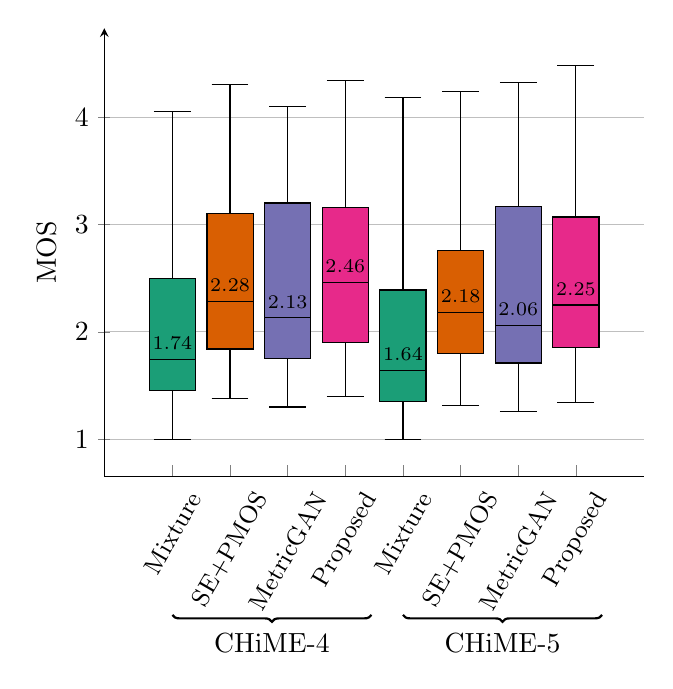
\begin{tikzpicture}
	\begin{axis}[
	    cycle list/Dark2-4,
		boxplot/draw direction = y,
		boxplot/box extend=0.8,
% 		x=3em,
% 		x axis line style = {opacity=0.6},
		axis x line* = bottom,
		axis y line = left,
		enlarge y limits,
		ymajorgrids,
		xtick = {1, 2, 3, 4, 5, 6, 7, 8},
		xticklabel style = {align=center, font=\small, rotate=60, alias={xtick-\ticknum}},
		xticklabels = {Mixture, SE+PMOS, MetricGAN, Proposed, Mixture, SE+PMOS, MetricGAN, Proposed},
% 		xtick style = {draw=none}, % Hide tick line
		ylabel = {MOS},
		ytick = {1, 2, 3, 4, 5},
	]
	
	\addplot+[
        boxplot prepared={
        lower whisker=1, lower quartile=1.45,
        median=1.74,
        upper quartile=2.5, upper whisker=4.05, }, fill, draw=black]
        coordinates {}
        node[above, color=black] at
        (boxplot box cs: \boxplotvalue{median},.5)
        {\scriptsize \pgfmathprintnumber{\boxplotvalue{median}}};
    \addplot+[
        boxplot prepared={
        lower whisker=1.38, lower quartile=1.84,
        median=2.28,
        upper quartile=3.1, upper whisker=4.3, }, fill, draw=black]
        coordinates {}
        node[above, color=black] at
        (boxplot box cs: \boxplotvalue{median},.5)
        {\scriptsize \pgfmathprintnumber{\boxplotvalue{median}}};
    \addplot+[
        boxplot prepared={
        lower whisker=1.3, lower quartile=1.75,
        median=2.13,
        upper quartile=3.2, upper whisker=4.1, }, fill, draw=black]
        coordinates {}
        node[above, color=black] at
        (boxplot box cs: \boxplotvalue{median},.5)
        {\scriptsize \pgfmathprintnumber{\boxplotvalue{median}}};
    \addplot+[
        boxplot prepared={
        lower whisker=1.4, lower quartile=1.9,
        median=2.46,
        upper quartile=3.16, upper whisker=4.34, }, fill, draw=black]
        coordinates {}
        node[above, color=black] at
        (boxplot box cs: \boxplotvalue{median},.5)
        {\scriptsize \pgfmathprintnumber{\boxplotvalue{median}}};
        
    \addplot+[
        boxplot prepared={
        lower whisker=1.0, lower quartile=1.35,
        median=1.64,
        upper quartile=2.39, upper whisker=4.18, }, fill, draw=black]
        coordinates {}
        node[above, color=black] at
        (boxplot box cs: \boxplotvalue{median},.5)
        {\scriptsize \pgfmathprintnumber{\boxplotvalue{median}}};
    \addplot+[
        boxplot prepared={
        lower whisker=1.31, lower quartile=1.8,
        median=2.18,
        upper quartile=2.76, upper whisker=4.24, }, fill, draw=black]
        coordinates {}
        node[above, color=black] at
        (boxplot box cs: \boxplotvalue{median},.5)
        {\scriptsize \pgfmathprintnumber{\boxplotvalue{median}}};
    \addplot+[
        boxplot prepared={
        lower whisker=1.26, lower quartile=1.71,
        median=2.06,
        upper quartile=3.17, upper whisker=4.32, }, fill, draw=black]
        coordinates {}
        node[above, color=black] at
        (boxplot box cs: \boxplotvalue{median},.5)
        {\scriptsize \pgfmathprintnumber{\boxplotvalue{median}}};
    \addplot+[
        boxplot prepared={
        lower whisker=1.34, lower quartile=1.85,
        median=2.25,
        upper quartile=3.07, upper whisker=4.48, }, fill, draw=black]
        coordinates {}
        node[above, color=black] at
        (boxplot box cs: \boxplotvalue{median},.5)
        {\scriptsize \pgfmathprintnumber{\boxplotvalue{median}}};
        
	\end{axis}
	
	\path (0,0) coordinate (P);
    \draw [thick,decoration={brace,mirror,raise=5em},decorate] (xtick-0|-P) -- (xtick-3.5|-P) 
        node[midway,yshift=-6em]{CHiME-4};
    \draw [thick,decoration={brace,mirror,raise=5em},decorate] (xtick-4|-P) -- (xtick-7.5|-P) 
        node[midway,yshift=-6em]{CHiME-5};

    % \node[text width=3cm] at (1.54,0.5) 
    % {\scriptsize 1.54};

\end{tikzpicture}

\caption{MOS ratings of the speech enhancement modes on CHiME-4 and CHiME-5 datasets using DNSMOS P.835.}
    % \vspace{-2em}
\label{fig:dnsmos_results}
    % \vspace{-0.4cm}
\end{figure}

\subsection{Perceptual quality evaluation}
\label{subsec:dnsmos}

We finally evaluate our model using P.835 metric~\cite{reddy2022dnsmos} to measure perceptual quality. We calculate the DNSMOS score on a scale of $[1-5]$ ($1$ = worst, $5$ = best) for the mixture, PMOS+SE, MetricGAN, and our proposed models using the CHiME-4~\cite{vincent2017analysis} and CHiME-5~\cite{barker2018fifth} datasets (simulated and real-recording). Figure~\ref{fig:dnsmos_results} shows the scores. With CHiME-4, the original mixture scores range from $1.45$ to $2.5$ with a median of $1.74$. Our proposed model achieves a median MOS of $2.46$, which is higher than the others. Fon CHiME-5, the original mixture scores range from $1.0$ to $4.18$. Our proposed model outperforms the others with a median of $2.25$. Our proposed model and PMOS+SE have smaller standard deviations compared to MetricGAN. Overall, our proposed model improves noisy speech in both the acoustic and perceptual aspects. 




% \subsection{Listening results}
% \label{subsec:listening_results}

% We conduct an IRB-approved listening study using Amazon Mechanical Turk to conceive the perceptual quality of enhanced speech assessed by normal-hearing listeners. 

% This study follows the design structure of \cite{nayem2021towards} and figure~\ref{fig:survey} shows the actual listener study interface of a single question. The study is conducted as follows, the participant will listen to two audio signals, one is enhanced and the other is clean audio as reference.  Then they provide a preference score using a Likert scale. The scale ranges from $-3$ to $+3$, where $-3$ refers to a strong preference towards the first signal, $+3$ refers to a strong preference towards the second signal, and $0$ refers to no preference. Before providing a score, the participant can listen to the signals as many as times they like, where the scores are not limited to integer values. The two signals are randomly selected, and the participant listens to different audio clips in each question. The audio clips are chosen from the CHiME-5 and CHiME-4 corpus spoken by both males and females in equal proportion. Prior to actual survey questions, each participants has to pass eligibility test and make themselves familiar with the upcoming study session by going through a practice session. The structure of this practice session is similar to the actual study, however, speakers' voice and audio clips which participants hear in practice session are not used in the actual study. A tentative feedback is provided in the practice session to give a guideline to the participants, however, to avoid biases and leading answers, the feedback is provided in a form of range where the expected answer should reside.



%  \begin{figure}[thb!]
%     \centering
%     \includegraphics[width = 0.5\linewidth]{IEEEtran/figs/survey.png}
%     % \vspace{-2em}
%     \caption{A question of actual listener study interface conducted on MTurk.}
%     \label{fig:survey}
%     % \vspace{-2em}
% \end{figure}

% \nayem{***One paragraph on the statistics of the conducted study.}
% The study session contains total 30 questions, which is preceded by a practice session of 7 questions. Ten participants (9 male, 1 female) who are native English speakers over the age of 18 participated, where a headset/headphone was required to be worn. On average, participants took 14 minutes to complete the study, they were given $\$3$ monetary incentive.


\section{Discussion}
\label{sec:discuss}

Our proposed model outperforms all comparison models on SI-SDR metrics for both seen and unseen datasets, without optimization of any of the models (Table \ref{tab:results_cosineVoices}, \ref{tab:results_chime}). This means that our approach improves speech quality by minimizing the distortion ratio when separated from the noise component. Additionally, our models yield the best MOS-LQO ratings on real-world captured audios (CHiME datasets, Table \ref{tab:results_chime}). These results are consistent with the findings of \cite{zezario2022deep, nayem2021incorporating} that incorporating embeddings from a speech assessment model improves SE performance, and the results of \cite{braun2022effect} that using MOS loss during model optimization leads to higher MOS-LQO scores. Our proposed approach achieves PESQ and ESTOI scores that are only slightly lower than those of the best-performing model, with a difference of only $0.03$ and $0.01$, respectively. This indicates that speech quality and intelligibility metrics are closely related to the subjective speech quality metric (MOS-LQO), and that these metrics can be improved without explicit optimization. Furthermore, our proposed model achieves the best average DNSMOS scores with low standard deviations on CHiME datasets (Figure \ref{fig:dnsmos_results}), indicating that it is effective in a wide range of real-world noise levels. This is a desirable quality for an effective SE model to be effective not only in high SNRs and limited noisy environments, but also in large SNR ranges and real-world conditions such as those offered by the CHiME dataset.

When comparing our proposed model that uses mse+sa+mos loss to the PMOS+SE model (as shown in Table \ref{tab:results_chime}), we can observe significant improvements in all performance metrics. As both models use the same loss function, the improvements are attributed to the incorporation of LM and the joint learning method. Moreover, we found that these two models exhibit similar performance on the MOS prediction (Table \ref{tab:mos_results}), indicating that the benefits of joint learning mostly impact the enhancement part of the model.

An intriguing finding is that our proposed model shows a decline in WER\% when MOS loss is incorporated, especially for larger real-world recordings such as CHiME-5, with degradation up to $1.1$. Although our study is not primarily concerned with ASR performance, this suggests a potential trade-off between ASR accuracy and subjective speech quality scores. Further investigation is needed to comprehend this relationship.

Our proposed method demonstrates that training a speech enhancement (SE) model and a MOS-based speech assessment model jointly can lead to better speech quality measured by objective metrics such as perceptual quality, intelligibility, and MOS ratings. However, we acknowledge that our study's use of subjective MOS (sMOS) estimation instead of actual human listeners may introduce discrepancies between MOS-LQO and human-rated MOS, which could impact our findings. To address this limitation, we plan to conduct sMOS evaluation by human listeners in future work. Although we used the same MOS prediction model for all comparison models, we believe that incorporating human-rated sMOS evaluations will provide more robust insights into our proposed method's effectiveness.
For computing loss terms, we opt for the MSE loss function along with a bi-gram language model that considers only time-along transitions. Our aim is to keep the model simple and focus on the effectiveness of our approach. However, we acknowledge that using different loss functions for different loss components and employing a more complex language model that considers both temporal and spectral transition levels can be beneficial. We plan to explore these possibilities in our future work.



\section{Discussion and Limitations}

Although we can ablate concepts efficiently for a wide range of object instances, styles, and memorized images, our method is still limited in several ways. First, while our method overwrites a target concept, this does not guarantee that the target concept cannot be generated through a different, distant text prompt. We show an example in \reffig{limitation} (a), where after ablating {\menlo Van Gogh}, the model can still generate {\menlo starry night painting}. However, upon discovery, one can resolve this by explicitly ablating the target concept {\menlo starry night painting}. Secondly, when ablating a target concept, we still sometimes observe slight degradation in its surrounding concepts, as shown in \reffig{limitation} (c). 

\nupur{Our method does not prevent a downstream user with full access to model weights from re-introducing the ablated concept~\cite{ruiz2022dreambooth,kumari2022multi,gal2022image}. Even without access to the model weights, one may be able to iteratively optimize for a text prompt with a particular target concept. Though that may be much more difficult than optimizing the model weights, our work does not guarantee that this is impossible.}

Nevertheless, we believe every creator should have an ``opt-out'' capability. We take a small step towards this goal, creating a computational tool to remove copyrighted images and artworks from large-scale image generative models.



% \newpage
% references section
%
\bibliographystyle{IEEEtran}
\bibliography{0_main.bbl}



% biography section
%
\begin{IEEEbiography}
[{\includegraphics[width=1in,height=1.25in,clip,keepaspectratio]{figs/Khandokar_Nayem_profile_2}}]{Khandokar Md. Nayem} (Student Member, IEEE)
received the B.Sc. degree in computer science and engineering from the Bangladesh University of Science and Engineering, Dhaka, Bangladesh, in 2014 and the M.Sc. degree in computer science from the Indiana University, Bloomington, IN, USA, in 2019, where he is currently working toward the Ph.D. degree in computer science. His research interests include speech enhancement/processing, deep learning, and human speech perception.
\end{IEEEbiography}


\begin{IEEEbiography}
[{\includegraphics[width=1in,height=1.25in,clip,keepaspectratio]{figs/Donald_Williamson_profile}}]{Donald S. Williamson} (Senior Member, IEEE)
received the B.E.E. degree in electrical engineering from the University of Delaware, Newark, DE, USA, the M.S. degree in electrical engineering from Drexel University, Philadelphia, PA, USA, and the Ph.D. degree in computer science and engineering from The Ohio State University, Columbus, OH, USA. He is currently an Associate Professor with the Department of Computer Science and Engineering, Ohio State University, Columbus, OH, USA. His research interests include speech enhancement/separation, speech assessment, and audio privacy.
\end{IEEEbiography}

\end{document}


